% ------------------------------------------------------------------------
% ------------------------------------------------------------------------
% abnTeX2: Modelo de Trabalho Academico (tese de doutorado, dissertacao de
% mestrado e trabalhos monograficos em geral) em conformidade com
% ABNT NBR 14724:2011: Informacao e documentacao - Trabalhos academicos -
% Apresentacao
% ------------------------------------------------------------------------
% ------------------------------------------------------------------------
\documentclass[
	% -- opções da classe memoir --
	12pt,				% tamanho da fonte
	openright,			% capítulos começam em pág ímpar (insere página vazia caso preciso)
	onside,			% para impressão em recto e verso. Oposto a oneside
	a4paper,			% tamanho do papel.
	% -- opções da classe abntex2 --
	%chapter=TITLE,		% títulos de capítulos convertidos em letras maiúsculas
	%section=TITLE,		% títulos de seções convertidos em letras maiúsculas
	%subsection=TITLE,	% títulos de subseções convertidos em letras maiúsculas
	%subsubsection=TITLE,% títulos de subsubseções convertidos em letras maiúsculas
	% -- opções do pacote babel --
	english,			% idioma adicional para hifenização
	brazil				% o último idioma é o principal do documento
	]{abntex2}

% ---
% Pacotes básicos
% ---
\usepackage{lmodern}			% Usa a fonte Latin Modern
\usepackage[T1]{fontenc}		% Selecao de codigos de fonte.
\usepackage[utf8]{inputenc}		% Codificacao do documento (conversão automática dos acentos)
\usepackage{lastpage}			% Usado pela Ficha catalográfica
\usepackage{indentfirst}		% Indenta o primeiro parágrafo de cada seção.
\usepackage{color}				% Controle das cores
\usepackage{graphicx}			% Inclusão de gráficos
\usepackage{microtype} 			% para melhorias de justificação
\usepackage{tikz}
\usepackage{wrapfig}
% add to latexmk > http://tex.stackexchange.com/questions/105943/latexmk-and-nomencl
\usepackage[portuguese]{nomencl}
\makenomenclature
% ---

\newcommand{\subfigureautorefname}{\figureautorefname} % resolve problema autoref subfig

\usepackage[labelfont=bf]{caption}

\makeatletter
\@ifundefined{showcaptionsetup}{}{%
 \PassOptionsToPackage{caption=false}{subfig}}
\usepackage{subfig}
\makeatother

% ---
% Pacotes adicionais, usados apenas no âmbito do Modelo Canônico do abnteX2
% ---
\usepackage{lipsum}				% para geração de dummy text
% ---

% ---
% Pacotes de citações
% ---
\usepackage[brazilian,hyperpageref]{backref}	 % Paginas com as citações na bibl
\usepackage[alf,abnt-emphasize=bf]{abntex2cite}	% Citações padrão ABNT

% ---
% CONFIGURAÇÕES DE PACOTES
% ---

% ---
% Configurações do pacote backref
% Usado sem a opção hyperpageref de backref
\renewcommand{\backrefpagesname}{Citado na(s) página(s):~}
% Texto padrão antes do número das páginas
\renewcommand{\backref}{}
% Define os textos da citação
\renewcommand*{\backrefalt}[4]{
	\ifcase #1 %
		Nenhuma citação no texto.%
	\or
		Citado na página #2.%
	\else
		Citado #1 vezes nas páginas #2.%
	\fi}%
% ---

% ---
% Informações de dados para CAPA e FOLHA DE ROSTO
% ---
\titulo{Desenvolvimento de um sistema de resposta em sala de aula para auxiliar
o ensino e aprendizagem}
\autor{Pedro Henrique Araújo Sobral}
\local{Juazeiro, Bahia, Brasil}
\data{2016, v-0.0.1}
\orientador{Dr. Max Santana Rolemberg Farias}
% \coorientador{João Carlos Sedraz Silva}
\instituicao{%
  \textsc{Universidade Federal do Vale do São Francisco} -- UNIVASF
  \par
  \textsc{Colegiado de Engenharia de Computação}
 % \par
 }
\tipotrabalho{Trabalho de Conclusão de Curso}
% O preambulo deve conter o tipo do trabalho, o objetivo,
% o nome da instituição e a área de concentração
\preambulo{
Trabalho de conclusão de curso \mbox{apresentado} a
Universidade Federal do Vale do São \mbox{Francisco},
Campus Juazeiro, como requisito da obtenção do
título de Engenheiro de \mbox{Computação}.}
% ---


% ---
% Configurações de aparência do PDF final

% alterando o aspecto da cor azul
\definecolor{blue}{RGB}{41,5,195}

% informações do PDF
\makeatletter
\hypersetup{
   	%pagebackref=true,
		pdftitle={\@title},
		pdfauthor={\@author},
  	pdfsubject={\imprimirpreambulo},
    pdfcreator={LaTeX with abnTeX2},
		pdfkeywords={abnt}{latex}{abntex}{abntex2}{trabalho acadêmico},
		colorlinks=true,       		% false: boxed links; true: colored links
  	linkcolor=blue,%blue,          	% color of internal links
  	citecolor=blue,%blue,        		% color of links to bibliography
  	filecolor=magenta,%magenta,      		% color of file links
		urlcolor=blue,%blue,
		bookmarksdepth=4
}
\makeatother
% ---

% ---
% Espaçamentos entre linhas e parágrafos
% ---

% O tamanho do parágrafo é dado por:
\setlength{\parindent}{1.3cm}

% Controle do espaçamento entre um parágrafo e outro:
\setlength{\parskip}{0.2cm}  % tente também \onelineskip

% ---
% compila o indice
% ---
% \makeindex
% --

\newcommand{\clicker}{\textit{clicker}}
\newcommand{\clickers}{\textit{clickers}}


\includeonly{
  % pretextual/fichacatalografica,
  % pretextual/errata,
  % pretextual/folhadeaprovacao,
  % pretextual/dedicatoria,
  % pretextual/agradecimentos,
  % pretextual/epigrafe,
  % pretextual/resumo,
  % pretextual/listas,
  textual/introducao,
  % textual/referencialteorico,
  % postextual/anexos,
  % postextual/apendice,
  % postextual/glosario,
  % postextual/indiceremissivo,
}

% ----
% Início do documento
% ----
\begin{document}

% Seleciona o idioma do documento (conforme pacotes do babel)
%\selectlanguage{english}
\selectlanguage{brazil}

% Retira espaço extra obsoleto entre as frases.
\frenchspacing

% ----------------------------------------------------------
% ELEMENTOS PRÉ-TEXTUAIS
% ----------------------------------------------------------
% \pretextual

% ---
% Capa
% ---
\imprimircapa
% ---

% ---
% Folha de rosto
% (o * indica que haverá a ficha bibliográfica)
% ---
\imprimirfolhaderosto*

\instituicao{%
  \textsc{Universidade Federal do Vale do São Francisco} -- UNIVASF
  \par
  \textsc{Colegiado de Engenharia de Computação}
}
% ---

% ---
% Inserir a ficha bibliografica
% ---
% \include{pretextual/fichacatalografica}

% ---
% Inserir errata
% ---
% \include{pretextual/errata}

% ---
% Inserir folha de aprovação
% ---
% Isto é um exemplo de Folha de aprovação, elemento obrigatório da NBR
% 14724/2011 (seção 4.2.1.3). Você pode utilizar este modelo até a aprovação
% do trabalho. Após isso, substitua todo o conteúdo deste arquivo por uma
% imagem da página assinada pela banca com o comando abaixo:
%
% \includepdf{folhadeaprovacao_final.pdf}
%
\begin{folhadeaprovacao}

  \begin{center}
    {\ABNTEXchapterfont\large\imprimirautor}

    \vspace*{\fill}\vspace*{\fill}
    \begin{center}
      \ABNTEXchapterfont\bfseries\Large\imprimirtitulo
    \end{center}
    \vspace*{\fill}

    \hspace{.45\textwidth}
    \begin{minipage}{.5\textwidth}
        \imprimirpreambulo
    \end{minipage}%
    \vspace*{\fill}
   \end{center}

   Trabalho \rule{2.5cm}{.2pt}. \imprimirlocal, 24 de Julho de 2017:

   \assinatura{\textbf{\footnotesize{Orientador (\textsc{CCOMP/UNIVASF)}}}\\ \imprimirorientador}
   \assinatura{\textbf{\footnotesize{Professor (CCOMP/UNIVASF)}} \\ Dr. Brauliro Gonçalves Leal}
   \assinatura{\textbf{\footnotesize{Professor (CCIVIL/UNIVASF)}} \\ Me. João Carlos Sedraz Silva}

   \begin{center}
    \vspace*{0.5cm}
    {\large\imprimirlocal}
    \par
    {\large\imprimirdata}
    \vspace*{1cm}
  \end{center}

\end{folhadeaprovacao}
% ---


% ---
% Dedicatória
% ---
% \include{pretextual/dedicatoria}

% ---
% Agradecimentos
% ---
% \include{pretextual/agradecimentos}

% ---
% Epígrafe
% ---
\begin{epigrafe}
    \vspace*{\fill}
	\begin{flushright}
    \textit{
    ``Diga-me eu esquecerei,\\
        ensina-me e eu poderei lembrar,\\
        envolva-me e eu aprenderei.''\\
        (Benjamin Franklin)}
	\end{flushright}
\end{epigrafe}
% ---


% ---
% RESUMOS
% ---
% resumo em português
\setlength{\absparsep}{18pt} % ajusta o espaçamento dos parágrafos do resumo
\begin{resumo}
  Este trabalho apresenta um breve estudo sobre o aprendizado ativo

  Nesse trabalho de conclusão de curso será desenvolvido um sistema de resposta em sala de aula,
  que possibilite aos professores e aos estudantes uma ferramenta de software livre,
  que permita usar {\textit{smartphones}} como {\clickers} para que o mesmo possa
  ser usado principalmente com práticas pedagógicas de aprendizado ativo como o \textit{Peer Instruction}.
 % O resumo deve ressaltar o
 % objetivo, o método, os resultados e as conclusões do documento. A ordem e a extensão
 % destes itens dependem do tipo de resumo (informativo ou indicativo) e do
 % tratamento que cada item recebe no documento original. O resumo deve ser
 % precedido da referência do documento, com exceção do resumo inserido no
 % próprio documento. (\ldots) As palavras-chave devem figurar logo abaixo do
 % resumo, antecedidas da expressão Palavras-chave:, separadas entre si por
 % ponto e finalizadas também por ponto.

 \textbf{Palavras-chave}:  Aprendizado Ativo. Instrução pelos Colegas. Sistemas de Resposta em Sala de Aula. Aplicativos Híbridos para Celular.
\end{resumo}

% resumo em inglês
\begin{resumo}[Abstract]
 \begin{otherlanguage*}{english}


   \vspace{\onelineskip}

   \noindent
   \textbf{Keywords}: Active Learning. Peer Instruction. Classroom Response Systems. Hybrid Mobile Applications.
 \end{otherlanguage*}
\end{resumo}


% ---
% LISTAS
% ---
\include{pretextual/listas}


% ----------------------------------------------------------
% ELEMENTOS TEXTUAIS
% ----------------------------------------------------------
\textual
% ---
\chapter{Introdução}

Por que ainda se justifica o modelo de ensino em que se baseia
na disseminação de informações, que nunca foi tão fácil achar (internet,
livros, etc)? O ensino de hoje deveria estar focado para uma nova
visão em que o papel do professor seja de intermediar a aprendizagem \cite{Araujo2013}.

Nesse modelo de ensino, o construtivismo, os estudantes são agentes ativos do próprio processo
de ensino e construção do conhecimento. Uma aplicação prática desse modelo teórico de ensino é o aprendizado ativo.
O aprendizado ativo é um conjunto de práticas pedagógicas que além de envolver os estudantes no
fazer, os faça pensar no que estão fazendo, ou seja, além de ouvir, eles precisam ler,
escrever, discutir, ou estarem envolvidos na resolução de problemas \cite{Charles1991}.

Uma metodologia de aprendizado ativo que tem alcançado sucesso internacionalmente é
a Instrução pelos Colegas (IpC) ou \textit{peer instruction} \cite{Araujo2013}. Resumidamente,
o IpC promove o aprendizado ativo com questionamentos regulares na aula, fazendo com que os
estudantes passem mais tempo discutindo e pensando sobre um conteúdo, do que assistindo passivamente a aula.

Assim como no modelo de ensino tradicional, a tecnologia também pode ser usada para promover
de forma mais eficiente o aprendizado ativo. No caso do IpC, a etapa fundamental de votação de uma questão
(apresentado em detalhes no \autoref{chap:revision}, \autoref{section:ipc}),
o uso de sistemas de resposta permitem ao professor uma análise posterior dos resultados,
além de dinamizar o processo de votação em sala de aula.

Sistemas de respostas são sistemas que possibilitam que todos os alunos
respondam a questões apresentadas pelo professor. Geralmente um gráfico de barras
é apresentado logo em seguida que os estudantes submetem as suas soluções
utilizando algum dispositivo remoto também conhecido como \textit{clickers}. As respostas são anônimas para os seus colegas,
no entanto o professor pode identificar cada estudante individualmente pela
identificação única do dispositivo, permitindo assim uma análise individual \cite{Kay2009}.
O resultado imediato disponibilizado por tais sistemas pode ser usado juntamente
com metodos que promovem a interação social voltada para a aprendizagem como o IpC.

Não existe na literatura um consenso sobre a nomenclatura para referenciar sistemas de
resposta para uso em sala de aula. Pode-se encontrar termos como
{\textit{``student response system''}} (sistema de resposta do estudante),
{\textit{``audience response system''}} (sistema de resposta a audiência),
{\textit{``personal response systems''})} (sistema de resposta pessoal),
{\textit{``classroom response systems''} (CRS)\nomenclature{CRS}{Classroom Response System}} (sistemas de resposta em sala de aula),
ou apenas como {``\clickers''} \cite{Hunsu2016}.
Nesse trabalho, para simplificação foi utilizado apenas a sigla {\clicker} ({\textit{Classroom Response System})
para referenciar esse tipo de sistema.

O uso de CRS associado com um modelo de aprendizado ativo mostrado
trazer vários benefícios para a sala de aula, como aumento na frequência escolar \cite{Fotaris2016},
melhora na atenção dos estudantes \cite{Terrion2012} e maior engajamento da turma \cite{Kaya2016}.
Também promove benefícios para a aprendizagem com um aumento na interação e discussão na sala de aula \cite{Mattos2015, Barragues2011},
e com melhora no aprendizado \cite{sun2014, Hunsu2016}. Além dos
benefícios para avaliação pelo \textit{feedback} imediato do entendimento dos estudantes
sobre um determinado conteúdo  \cite{Rana2016, Blood2013}.

Apesar dos benefícios significativos do uso associado com CRS na sala de aula,
o preço de tais tecnologias podem representar um custo econômico considerável
para instituições de ensino, que pode se tornar uma barreira para adoção de CRS e
adotá-las no processo de aprendizagem \cite{Blasco-Arcas2013}.

Nesse sentido, considerando que os \textit{smartphones} podem ser usados
como parte integrante dos CRSs como o dispositivo em que os estudantes vão submeter as respostas (ou \textit{clickers}),
e da quase ubiquidade de tais dispositivos entre os jovens brasilieiros - já em 2014 mais de 93\% dos estudantes da rede
privada de ensino e quase 65\% dos da rede pública possuem \textit{smartphones} \cite[p. 55]{IBGE2016} -,
este trabalho apresenta o desenvolvimento de um CRS de software livre que permita usar
{\textit{smartphones}} como \textit{clickers}.

\section{Objetivo Geral}
Desenvolver um sistema de resposta para uso sala de aula (CRS),
que possibilite aos professores e aos estudantes uma ferramenta de software livre,
que permita usar {\textit{smartphones}} como \textit{clickers}.

\section{Objetivos Específicos}

\begin{itemize}
    \item Realizar levantamento de requisitos sobre os sistemas de resposta em sala de aula;
    \item Especificar e implementar uma aplicação para dispositivos móveis, que será utilizado como \textit{clickers};
    \item Especificar e implementar uma aplicação web para o professor administrar as questões e gerar relatórios;
    \item Especificar e implementar um sistema servidor, para receber e
    enviar dados para os os clientes: dispositivos móveis dos alunos e navegador
    web do professor.
\end{itemize}

\section{Organização do texto}
Além desta introdução, este trabalho está dividido em mais quatro capítulos.

\begin{description}
  \item[Revisão de literatura:] Esse capítulo discute um contexto pedagógico
  para o uso de sistemas de resposta em sala de aula. Inicialmente, é
  apresentado o conceito de aprendizado ativo e um método de implementação: Instrução pelos Colegas.
  Em seguida, são apontados os sistemas de resposta em sala de aula como uma
  ferramenta para ajudar o professor a mediar um aprendizado significativo  em
  sala de aula. O capítulo é encerrado apresentando os benefícios e desafios de uso dessa tecnologia.

  \item[Engenharia de Software:] Nesse capítulo são descritas as fases de especificação, projeto, implementação e testes do sistema.
  Os procedimentos, material e métodos, resultados e discussões e cada etapa também é apresentado nesse capítulo.

  \item[Resposta em Sala de Aula:] Nesse capítulo é apresentado o software desenvolvido,
  definições, as principais telas e característica do sistema desenvolvido.

  \item[Considerações finais e trabalhos futuros:] São realizadas as considerações finais do
  trabalho e apontadas diretrizes para trabalhos futuros.

\end{description}

\chapter{Revisão de Literatura}
\begin{quote}\normalfont\itshape\vspace*{-2\baselineskip}
  Neste capítulo, inicialmente, é
  apresentado o conceito de aprendizado ativo e uma alternativa para a implementação dessa
  metodologia de ensino.
  Em seguida, é apontado o {\clicker} como uma
  ferramenta para ajudar o professor na promoção de um aprendizado significativo  em
  sala de aula. O capítulo é encerrado com informações sobre os benefícios e desafios de uso de dessa tecnologia.
\end{quote}


\section{Aprendizado Ativo}\label{section:aprendizado_ativo}
Em resumo, o aprendizado ativo é um conjunto de práticas pedagógicas
que além de envolver os estudantes no fazer, os faça pensar no que estão fazendo \cite[p. 19]{Charles1991}.

Os princípios do aprendizado ativo são dois: introduzir atividades nas salas de aula
tradicionais e promover o envolvimento dos estudantes. O primeiro é a forma
mais simples do aprendizado ativo. Um exemplo seria fazer pequenas pausas na aula
e colocar os estudantes para revisar as notas de aula com um colega. No entanto,
é preciso que tais atividades promovam o engajamento dos estudantes no processo
de ensino e aprendizagem \cite[p. 3]{Prince2004}.

Em salas de aula que utilizam o aprendizado ativo pode-se ter um aumento de até 6\%
na média final nas provas dos alunos e que aquelas salas de aula puramente expositivas
têm 55\% mais chance de reprovarem os alunos do que aquelas com aprendizado ativo.
Esse aumento que pode parecer pouco (0,3 na média final) colocaria a média daqueles estudantes
que desistem do curso bem próximo daqueles que permanecem, podendo-se dessa forma aumentar
a taxa de retenção dos estudantes \cite[p. 4]{Freeman2014}.

O estudo de meta-análise de \citeonline{Freeman2014} envolveu mais de 200 artigos,
que comparavam as performances dos alunos em salas de aula com pelo menos algum
elemento de aprendizado ativo com as tradicionais aulas expositivas. Além de
mostrarem evidências de que o aprendizado ativo pode melhorar o aprendizado dos
estudantes de graduação, principalmente nas áreas de ciência, tecnologia, engenharia
e matemática, \citeauthoronline{Freeman2014} propõem aos futuros pesquisadores
testarem não mais a eficiência dos métodos de aprendizado ativo frente as tradicionais
aulas expositivas (``primeira geração de pesquisas''), mas sim qual
o tipo de aprendizado ativo é mais apropriado para cada área do conhecimento
(``segunda geração de pesquisas'').


Apesar dos indícios dos benefícios da Aprendizagem Ativa, no contexto brasileiro,
tornar o aluno um agente ativo no processo de ensino e aprendizagem não é uma tarefa fácil.
São muitas as adversidades de infraestrutura e institucionais
encontradas de modo a propiciar o desenvolvimento dessa metodologia. Seja por salas com
numero excessivo de alunos, estes desinteressados, professores mal pagos, ou com
a pressão de produzir cientificamente \cite{Araujo2013}.

Por outro lado, muitas são as iniciativas encontradas na literatura mostrando resultados
satisfatórios que podem ajudar o professor nesse processo \cite{Crouch2001, Gok2013, Barros2004}.
Na próxima seção será apresentado o método ativo de ensino \textit{Peer Instruction} ou \textit{Instrução pelos Colegas}
(IpC)\nomenclature{IpC}{Instrução pelos Colegas}.

\subsection{Instrução pelos Colegas (IpC)}
\label{section:ipc}

O IpC foi desenvolvido pelo Professor Eriz Mazur da Universidade de Harvard (EUA)\nomenclature{EUA}{Estados Unidos da América} na
década de 1990. O objetivo do IpC é fazer com que todos os estudantes se engajem em
discussões com o vizinho de opinião diferente sobre um determinado conceito e fazer com que cada
estudante tente explicar o conceito um para o outro \cite{Mazur2009}.

No método IpC, geralmente, o professor começa fazendo uma breve exposição dialogada do conteúdo (15min).
Depois é colocado para os estudantes uma questão conceitual, que é
desenvolvida de modo a avaliar o entendimento dos estudantes sobre um tópico.
A \autoref{fig:desen_fluxograma_ipc} resume o processo de implementação do método IpC na sala de aula.

\begin{figure}[b]
  \centering
  \caption{Diagrama do processo de implementação do método IpC}
  \includegraphics[clip, trim=0cm 18cm 3cm .4cm, width=.85\textwidth]{imagens/peer_instruction}
  \label{fig:desen_fluxograma_ipc}
  \fonte{Adaptado de \cite{Araujo2013}}
\end{figure}

Um exemplo de uma questão conceitual de introdução a física é mostrada na \autoref{fig:desenv_ct}. Os
estudantes respondem individualmente  a questão (1-2min), geralmente, utilizando
\textit{clickers}, que são pequenos dispositivos transmissores como os da \autoref{fig:desenv_clickers}.
Em seguida, dependendo do percentual de alunos que acertem a questão,
o professor pode revisar o assunto (acerto < 30\%), fazer uma breve explanação da
questão e ir para um próximo tópico ou nova questão (acerto > 70\%), ou o que se
deseja do método, um percentual de acerto entre 30\% e 70\% em que, nessa situação, o
professor estimula que os alunos encontrem um parceiro que respondeu de forma diferente
e que tentem explicar um para o outro o porquê de estar correto. Com esse processo, os alunos se auto
instruem, o que justifica o nome do método ``Instrução pelos Colegas'' \cite{Mazur2009, Crouch2001}.


\begin{figure}[t]
  \centering
  \caption{Exemplo de uma questão conceitual}
  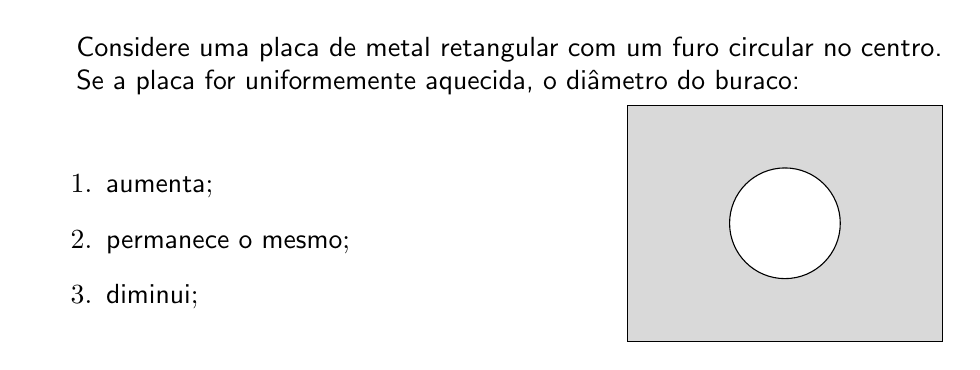
\begin{tikzpicture}[scale=1]
    \label{fig:desenv_ct}
    \node[,text width=11cm] at (0,4) {\textsf{Considere uma placa de metal retangular com um furo circular no centro. Se a
    placa for uniformemente aquecida, o diâmetro do buraco:}};
    \node[,text width=5cm] at (-3.5,2) {
      \begin{enumerate}
        \item \textsf{aumenta};
        \item \textsf{permanece o mesmo};
        \item \textsf{diminui};
      \end{enumerate}
    };
    \draw[fill=gray!30, shift={(1.5cm,.5cm)}](0,0) rectangle (4,3);
    \draw[fill=white, shift={(1.5cm,.5cm)}](2,1.5) circle(20pt);
  \end{tikzpicture}
  \fonte{Adaptado de \cite{Watkins2013}}
\end{figure}

Uma das etapas do IpC na sala de aula é a votação, em que os estudantes indicam
as suas respostas. Existem pelo menos quatro maneiras \cite{Crouch2007} do professor
obter um \textit{feedback} da votação dos estudantes:

\begin{description}
  \item[Levantar as mãos:] a forma mais simples é pedir para os alunos levantarem as mãos para cada alternativa,
  mas, dentre as várias limitações desse método, os estudantes podem se influenciar pela resposta dos outros.
  \item[Cartões coloridos:] uma segunda alternativa seria o uso de
  cartões coloridos (\textit{flashcards}) que dificultaria os alunos ver a resposta
  dos outros e facilitaria a contagem pelo professor, porém uma limitação desse método,
  assim como o anterior é a dificuldade de alguma forma guardar os resultados.
  \item[Folha de respostas:] outra alternativa, no entanto não seria possível ter
  um resultado imediato das respostas.
  \item[Sistemas de resposta em sala de aula:] exemplo os \textit{clickers} da \autoref{fig:desenv_clickers}, ou \textit{smartphones},
  e sistemas web possibilitam aos estudantes enviarem imediatamente as respostas ao
  computador do professor, de forma anônima aos colegas de sala e visualizar graficamente
  os resultados.
\end{description}


\begin{figure}
  \begin{centering}
    \caption{\label{fig:desenv_clickers}Exemplo de \textit{clickers}}
    \subfloat[\textit{i>clicker 2}]{\includegraphics[scale=0.25]{imagens/desenv_iclicker}\label{fig:clickersA}}
    \hspace{.5cm}
    \subfloat[\textit{ResponseCard RF LCD}]{\includegraphics[scale=.4517]{imagens/desenv_turning_clicker}}
    \par
  \end{centering}
  \fonte{(a) \href{http://www1.iclicker.com}{iclicker.com} (b) \href{http://www.turningtechnologies.com}{turningtechnologies.com}}
\end{figure}

% No entanto, a implementação do IpC não ocorre apenas na sala de aula. Espera-se
% que os alunos façam leituras e atividades antes da aula. Também espera-se do
% professor guiar os estudantes nessa etapa, seja indicando ou disponibilizando o
% material adequado. O tempo em sala de aula que seria utilizado para apenas transferir
% informações para os estudante é utilizado principalmente para discussões, interação
% entre os estudantes, tempo para assimilação e para pensar \cite{Mazur2009, Crouch2001}.




\section{Sistemas de Resposta em Sala de Aula}
\label{section:sistemas_de_resposta}

Sistemas de respostas em sala de aula são tecnologias que permitem ao professor
realizar questionamentos a toda classe e, assim, obter o resultados das respostas
em tempo real \cite{Kay2009}. Geralmente, as questões são no formato de verdadeiro ou
falso e questões de múltipla escolha. Tais sistemas também podem ser usados para
saber a impressão dos alunos sobre um determinado tema \cite{Fies2006}.

Inicialmente introduzido em 1966 na Universidade de Stanford (EUA), os sistemas
de resposta não funcionavam direito, eram difíceis de usar e caros \cite{Kay2009}. Dispositivos
de coleta de respostas como os da \autoref{fig:desenv_clickers} que usam infravermelho, com preços mais
atrativos, começaram a ser extensivamente usados a partir de 2003 e hoje existe pelo menos
uma disciplina em cada universidade dos Estados Unidos em que se faz uso de tais sistemas
no processo de ensino e aprendizagem \cite{Abrahamson2014}.

Entretanto, ainda que o custo individual de um aparelho seja atrativo para um
estudante, a realidade da universidade pública brasileira é diferente em relação
a dos Estados Unidos. Assim como não existe obrigatoriedade do aluno comprar um
livro-texto no Brasil, também não existe mecanismo que os faça
comprar \textit{clickers} \cite{GerdKortemeyerEmersonCruz2011}. Dessa forma, os \textit{clickers}
teriam que ser comprados pela universidade, e o custo total não seria tão atrativo.

Por exemplo, a Universidade de São Paulo (USP)\nomenclature{USP}{Universidade de São Paulo}, em uma tentativa pioneira de
\citeonline{GerdKortemeyerEmersonCruz2011} de oferecer oportunidades para a avaliação
formativa usando \textit{clickers} como os da \autoref{fig:clickersA} em duas
turmas de física, com 80 alunos cada. Com cada \textit{i>clicker 2}
custando \$43,74 (\autoref{fig:desenv_preco})
o valor total apenas dos 160 \textit{clickers} seria de
R\$22.116,34\footnote{Considerando o valor do dólar comercial em 12. Ago. 2016
de R\$3,1602. Disponível em: \href{http://www4.bcb.gov.br/pec/taxas/port/ptaxnpesq.asp?id=txcotacao}{http://www4.bcb.gov.br/pec/taxas/port/ptaxnpesq.asp?id=txcotacao}},
necessitando para compor o sistema, ainda, o aparelho que recebe as respostas, software que é instalado
no computador do professor, treinamento e suporte, ou seja, o valor final pode ser
ainda maior. Esse elevado valor de aquisição dos {\clickers}, é uma das principais barreiras na adoção dessa
ferramenta no processo de ensino, que ainda tem a resistência de alguns professores
em usar novas tecnologias como ferramentas de ensino \cite{Moratelli2014, Blasco-Arcas2013, Strasser2010, GerdKortemeyerEmersonCruz2011, Kay2009}.

\begin{figure}[!t]
  \centering
  \caption{Preço do \textit{i>clicker 2}}
  \includegraphics[width=.75\textwidth]{imagens/desenv_preco}
  \fonte{\href{https://goo.gl/q4nBdg}{amazon.com} pesquisando \textit{i>clicker 2}. Acesso em 12. Ago. 2016}
  \label{fig:desenv_preco}
\end{figure}

Todavia, uma maneira de tornar tal tecnologia mais acessível é usar os próprios
celulares dos estudantes como {\clickers} \cite{Stowell2015, Morrell2015, Araujo2013}.
Além de mais acessível, usando os próprios celulares, os estudantes podem
ver as questões e os resultados da classe nos próprios aparelhos. Para o professor,
uma variedade maior de questões podem ser exploradas, como uma  questão aberta \cite{Stowell2015}.

Saliente-se ainda que, embora possa haver um pequeno aumento no número de questões
sem respostas, as respostas dos estudantes são comparáveis quando se usa
\textit{clickers} \cite{Morrell2015, Stowell2015}.

Ainda que o uso do celular como {\clicker} possa aumentar o nível de
distrações, são muitos os benefícios de usar essa abordagem, no entanto,
é preciso estar atento aos pequenos casos de estudantes que não têm a tecnologia
adequada, ou que não queiram usar os seus dispositivos \cite{Morrell2015, Stowell2015}.

% \subsection{\textit{Smartphones} no Brasil}
%
% É importante aqui destacar o uso dos dispositivos que podem permitir essa abordagem
% na realidade brasileira. Hoje existem 1,2 dispositivos portáteis
% (\textit{smartphones} e \textit{tablets}) por habitante e uma projeção para o próximo
% biênio 2017/2018 de 2 dispositivos
% (desktops, \textit{notebooks}, \textit{tablets} e \textit{smartphones}) por habitante \cite[p. 8]{Meirelles2016}.
% Acrescenta-se também que já em 2014 mais de 93\% dos estudantes da rede privada de
% ensino e quase 67\% dos da rede pública possuem \textit{smartphones}, em que a
% proporção de pessoas é maior na rede pública \cite[p. 55]{IBGE2016}. Também cabe
% ressaltar que o celular já é o principal meio para acessar a Internet nos domicílios
% brasileiros \cite[p. 41]{IBGE2016}.

\subsection{Alternativas Disponíveis}
\label{subp:alternativas_disponiveis}

Em um estudo para desenvolver uma estratégia de ensino utilizando
{\clickers} como recurso didático, \citeonline{Mattos2015}, utilizou o
\href{https://www.polleverywhere.com/}{\textit{Poll Everywhere}}, que foi
escolhido principalmente por ser compatível com as principais plataformas
móveis (Android, iOS e Windows Phone). O
\href{https://www.polleverywhere.com/}{\textit{Poll Everywhere}} oferece uma
versão gratuita com no máximo 40 respostas por votação com algumas limitações.
Na versão paga, o estudante pode pagar \$14/ano ou o professor pode pagar
\$349/semestre (vide \autoref{fig:polleverywhere}).

Outra solução é o \href{http://www.socrative.com/}{\textit{Socrative}},
que também é compatível com todas as plataformas, e na sua versão gratuita
permite até 50 alunos por votação, questões de múltipla escolha, de verdadeira e falso,
resposta curta, \textit{quizzes}, etc \cite{socrative2016}. Alguns relatos do uso do
\href{http://www.socrative.com/}{\textit{Socrative}} em sala de aula para promover
a interatividade são encontrados em \cite{Kaya2016, Trindade2014}.
Uma opção interessante do \href{http://www.socrative.com/}{\textit{Socrative}}
é o \textit{Exit Ticket}, em que ao final da aula os estudantes respondem
a três perguntas. A primeira funciona como uma autoavaliação, perguntando
o quanto o estudante entendeu da aula, já as outras duas como identificação, que são o
nome do aluno e uma pergunta que o professor coloca no quadro, ou seja, teoricamente,
apenas os alunos presentes vão ser capazes de responder corretamente, servindo
então como um controle de frequência. Na versão paga o professor pode pagar \$49,99/ano (vide \autoref{fig:socrative}).

Por último, o aplicativo \href{http://www.tophat.com/}{\textit{TopHat}}, usado diariamente por
mais 500 instituições de ensino pelo mundo \cite{tophat2016}.
Para o professor, \href{http://www.tophat.com/}{\textit{TopHat}} permite incorporar
uma variedade de questões, uma revisão interativa da aula e para provas
\cite{Neilson2016, Lantz2014}. A inscrição mais popular no  \href{http://www.tophat.com/}{\textit{TopHat}}
são de \$36/ano (vide \autoref{fig:tophat}).

\begin{figure}
  \centering
  \caption{Preço de algumas sistemas de resposta}
  \subfloat[Disponível em: \href{https://www.polleverywhere.com/plans/higher-ed}{polleverywhere.com/plans/higher-ed}: em 16 ago. 2016]{
    \includegraphics[scale=0.35]{imagens/polleverywhere2}
    \label{fig:polleverywhere}
  }

  \subfloat[Disponível em: \href{http://www.socrative.com/pricing.php}{socrative.com/pricing}: em 16 ago. 2016]{
    \includegraphics[scale=0.35]{imagens/socrative}
    \label{fig:socrative}
  }

  \subfloat[Disponível em: \href{https://tophat.com/pricing/}{tophat.com/pricing} em: 16 ago. 2016]{
    \includegraphics[scale=0.35]{imagens/tophat}
    \label{fig:tophat}
  }
\end{figure}

\section{Benefícios dos Sistemas de Resposta em Sala de Aula}
Os benefícios do uso de sistemas de resposta em sala de aula podem ser divididos
em benefícios para a sala de aula, para a aprendizagem e para avaliação \cite{Kay2009}. As
subseções a seguir discutem cada tópico.

\subsection{Benefícios para a sala de aula}

\subsubsection{Frequência Escolar}
Não apenas uma ferramenta que também pode facilitar o controle de frequência
\cite{Strasser2010},
os sistemas de resposta em sala de aula têm sido utilizados com sucesso para aumentar
a frequência escolar \cite{Fotaris2016, Velasco2013, Puente2012, Mayer2009, Caldwell2007}. O fato dos
estudantes terem tido um retorno imediato das atividades que faziam interativamente
na sala de aula, pode ter contribuído para motivar os alunos para irem para as aulas \cite{Puente2012}.
Outro fator para o aumento da frequência é quando as questões dos {\clickers} contribuem na nota final,
em que o peso pode variar de 5\% a 15\% que o resultado parece ser o mesmo \cite{Caldwell2007}.

\subsubsection{Atenção}\label{subsubsection:attention}
Sabe-se hoje que a maioria das pessoas não conseguem se concentrar ininterruptamente
por mais de 20 min em uma única atividade \cite{Caldwell2007, DInverno2003}. Com aulas que
duram entre 2h-3h, os professores podem quebrar as aulas em miniaulas
com questões ao final delas usando os {\clickers} \cite{Hunsu2016}. Estudo de
ondas cerebrais mostraram que a atenção dos estudantes aumentam durante as
atividades de votação, além de reduzir a ansiedade \cite{Sun2014}. Acrescenta-se
também que quando os {\clickers} são adotados, os estudantes relatam a necessidade
de estudar antes da aula para participarem e prestarem atenção, dessa forma participam mais da aula \cite{Terrion2012}.

\subsubsection{Privacidade e Participação}\label{subsubsection:privacy}
Os estudantes podem responder as questões sem se preocupar com o julgamento
de seus colegas de classe ou do professor. Nesse ambiente seguro o estudante
não tem nenhuma razão para sentir medo de responder errado \cite{Schmidt2011}.
 A falta de privacidade pode coibir
a completa honestidade na votação \cite{Caldwell2007}, e a presença da mesma da a oportunidade
para os estudantes responderem e tomarem posições polêmicas em questões sensíveis \cite{Rana2016}.

\subsubsection{Engajamento}
Inúmeros estudos indicam estudantes mais interessados ou engajados no material
apresentado quando sistemas de resposta são usados
\cite{Kaya2016, Rana2016, Horne2015, Mattos2015, Moratelli2014, Kulatunga2014, Blood2013, Terrion2012,
Caldwell2007}.

\subsection{Benefícios para a aprendizagem}

\subsubsection{Interação e Discussão}
A interação na sala de aula é importante por três motivos: primeiro pelo que foi
apresentado na \autoref{subsubsection:attention}, segundo que permite clarificar
pontos obscuros e terceiro que permite uma monitoração do entendimento da classe
e velocidade do que é apresentado \cite{DInverno2003}. Nesse sentido, estudos
indicam aumento da interação na sala de aula \cite{Mattos2015, Barragues2011, Titman2011, Mayer2009, Caldwell2007}.

\subsubsection{\textit{Contingent Teaching}}\label{sussubsection:contingent}
\textit{Contingent Teaching} nada mais é do que a possibilidade de modificar
o curso do que está sendo ensinado com base no \textit{feedback} dos estudantes
\cite{Arnesen2013, Caldwell2007}. Por exemplo, se pouco mais da metade da classe
responde corretamente a uma questão, conclui-se uma falta de compreensão geral do
tópico apresentado, e assim o professor pode tentar explicar o conceito
de maneira diferente \cite{Terrion2012, Strasser2010}.

\subsubsection{Melhora no aprendizado}
\citeonline{Lantz2014} verificaram um aumento significativo (15\%) no grupo de
participantes que tiveram aulas com {\clickers} em relação ao sem o uso em testes que
ocorriam dois dias depois as aulas, e também permitiu aos estudantes corrigir
eventuais equívocos sobre o material de aula. Outros estudos apontam melhora
na performance dos estudantes \cite{Sun2014, Caldwell2007}. Entretanto, em um recente estudo de meta-análise,
em que se comparou classes que usaram e não usaram sistemas de resposta em sala de aula,
indicou um significativo impacto positivo nas variáveis cognitivas (retenção,
transferencia de conhecimento e sucesso), e nas variávies não-cognitivas (engajamento e participação, frequência, interesse,
percepção de qualidade) \cite{Hunsu2016}.

\subsection{Benefícios para avaliação}

\subsubsection{\textit{Feedback}}
Como destacado na \autoref{section:ipc}, dentre as quatro formas disponíves para
o professor obter um \textit{feedback} ou retorno do entendimento dos estudantes
sobre determinado tópico, se disponível, os {\clickers} são os mais eficazes \cite{Crouch2007}.
Os {\clickers} permitem um retorno imediato, preciso, privacidade (vide \autoref{subsubsection:privacy}) e
são divertidos de usar \cite{Rana2016, Blood2013, Caldwell2007}.

\subsubsection{Avaliação Formativa}
Avaliar o estudante permanemtemente, e não apenas utilizando avaliações pontuais,
não apenas classificar os alunos em os que sabem e os que não sabem, não apenas
verificar e sim avaliar, dedicar mais tempo nos erros \cite{UnivespTV2013}. Esses são alguns pontos
da avaliação formativa, que para o professor orienta a prática pedagógica, e para
o aluno permite uma autoavaliação sobre a aprendizagem \cite{Kay2009}. Os artigos
a seguir indicam que o uso de sistemas de resposta em sala de aula ajudam a
fornecer avaliações formativas eficazes \cite{Kortemeyer2016, Thampy2014, Kay2009, Fies2006}.

\subsection{Desafios para usar {\clickers}}
O uso dos {\clickers} também trazem alguns desafios, principalmente
tecnológicos ou estruturais e desafios centrado nos estudantes \cite{Cubric2015, Kay2009}.

\subsubsection{Tecnológicos/Estruturais}
\citeonline{Stowell2015} recomenda que as salas de aula tenham acesso confiável
a rede Wi-Fi, por isso o professor deve estar preparado quando a internet não
estiver disponível \cite{Strasser2010}. Como já abordado nesse trabalho (vide \autoref{section:sistemas_de_resposta}),
nem todos os estudantes vão ter a tecnologia adequada ou vontade de usar \cite{Morrell2015, Stowell2015}.
Dessa forma, \citeonline{Velasco2013} aconselham os {\clickers} como uma ferramenta opcional para
os estudantes.

\subsubsection{Desafio para os estudantes}
Alguns estudantes podem ter resistência ao novo, principalmente se já acomodados
a passividade em sala de aula \cite{Terrion2012, Kay2009}. Além disso, quando
usados apenas para controle de frequência, os estudantes podem ter uma percepção
negativa da tecnologia \cite{Terrion2012, Caldwell2007}.

\subsection{Considerações finais}
Por outro lado, apesar das seções anteriores serem animadoras quanto ao uso dos
{\clickers} é importante destacar a tecnologia apenas como um meio para
colaborar no processo de ensino e aprendizagem, e só faz sentido quando associada
com práticas pedagógicas de ensino como o aprendizado ativo
(vide \autoref{section:aprendizado_ativo}) \cite{Terrion2012, Moran2006}. O leitor interessado
sobre o uso das novas tecnologias em sala de aula, poderá buscar nas obras
indicadas em \cite{portalBrasil2014}.

\citeonline{Han2014} concluiu que o ensino e aprendizado com o auxílio de {\clickers}
ainda é um fenômeno complexo e relacional. Segundo o mesmo autor, estudos mais rigorosos
devem ser conduzidos para se entender por exemplo a relação entre o uso de {\clickers}
e o aprendizado, pois o benefícios da tecnologia podem variar pelo histórico do
estudante, motivação e metacognição.

% \chapter{Material e Métodos}
\chapter{Prototipação do Sistema}

\chapter{Resposta em Sala de Aula}

As principais tecnologias, ferramentas e métodos foram descritos nos capítulos
anteriores. Como resultado final foi desenvolvido um sistema de resposta
em sala de aula denominado \textit{Resposta em Sala de Aula}.

\section{Aplicação web para o Professor}

A \autoref{fig:main_window} ilustra a tela inicial da aplicação web para o professor.
Nela é possível perceber as três abas principais do sistema. A primeira \textit{Questões} que
está selecionada, permite ao professor gerir um banco de questões criadas, iniciar uma
sessão com questões selecionadas e categorizar as questões para uma melhor organização das mesmas.

\begin{figure}[ht]
  \centering
  \caption{Aba \textit{Questões}}
  \includegraphics[scale=.40]{imagens/telas/main_window}
  \doautor
  \label{fig:main_window}
\end{figure}

\subsection{Frequência dos alunos}
\label{sec:freq_students}

Um dos requisitos do sistema era permitir ao professor realizar a frequência dos alunos
pelo aplicativo. O sistema gera um código aleatório de quatro digitos e permite aos estudantes
submeterem esse código pelo aplicativo. O professor pode ativar a frequência
clicando no botão \textit{Frequência} no canto superior direito da aba \textit{Questões} (\autoref{fig:main_window}).
Em seguida, o sistema muda para a aba \textit{Ao Vivo}, tendo como resultado a \autoref{fig:live_freq}.
Nela é possível perceber o código de aleatório de quatro dígitos que foi gerado e alguns botões de ação no canto
inferior direto, permitindo ao professor encerrar a frequência por exemplo.

\begin{figure}[ht]
  \centering
  \caption{Página para a realizar a frequência dos estudantes}
  \includegraphics[scale=.45]{imagens/telas/live_freq}
  \doautor
  \label{fig:live_freq}
\end{figure}

Posteriormente, o professor pode acessar a lista de frequência por meio do aba \textit{Turmas},
clicando para cada turma a opção de \textit{atividades}, \autoref{fig:atividades}. A \autoref{fig:list_freq} exibe a
lista de frequência em detalhes.

\begin{figure}[ht]
  \centering
  \caption{Página para a realizar a frequência dos estudantes}
  \includegraphics[scale=.45]{imagens/telas/atividades}
  \doautor
  \label{fig:atividades}
\end{figure}

\begin{figure}[ht]
  \centering
  \caption{Página para a realizar a frequência dos estudantes}
  \includegraphics[scale=.45]{imagens/telas/list_freq}
  \doautor
  \label{fig:list_freq}
\end{figure}


\subsection{Cadastro de Questões}

A \autoref{fig:new_question} exibe o formulário para o cadastro de uma nova questão.
A aplicação permite a criação de questões de múltipla escolha, verdadeiro e falso e questão aberta.
Em questões do tipo múltipla escolha o professor deve indicar uma alternativa como correta.

\begin{figure}[ht]
  \centering
  \caption{Formulário \textit{Nova Questão}}
  \includegraphics[scale=.5]{imagens/telas/new_question}
  \doautor
  \label{fig:new_question}
\end{figure}

\subsection{Turmas}
\label{subsection:turmas}

Na aba de \textit{Turmas} (\autoref{fig:admin_classes}), o professor faz o cadastro das turmas
para permitir acesso aos estudantes. Foi criado o conceito de \textit{turmas públicas}
e \textit{turmas privadas}. Uma turma pública é aquele em que não existe uma
lista de alunos cadastrados, ou seja, qualquer aluno com o código de acesso da turma
vai poder acessar e participar das atividades apenas digitando o código de acesso.

Quando uma lista de estudantes é adicionada em uma turma (a \autoref{fig:add_students} ilustre esse processo) ela se
torna uma turma privada. Quando os estudantes acessarem a turma eles terão que
digitar além do código da turma, o código de identificação de cada um que foi cadastrado no sistema.

\begin{figure}[ht]
  \centering
  \caption{Aba \textit{Turmas}}
  \includegraphics[scale=.4]{imagens/telas/admin_classes}
  \doautor
  \label{fig:admin_classes}
\end{figure}

\subsubsection{Lista de estudantes em uma turma}

A \autoref{fig:add_students} ilustra o cadastro de estudantes de uma turma.
O professor tem a opção de adicionar manualmente cada estudante, clicando
na opção \textit{Adicionar manualemente} no canto inferior direito, digitando
o nome do estudante e o código de identificação (esse é o código que os estudantes
terão que digitar além do código da sala para ter acesso).

A outra opção para adicionar a lista de estudantes é importar um arquivo CSV
contendo o nome dos estudantes e código de identificação, clicando
na opção \textit{Importar Estudantes (CSV)} no canto inferior direito. Um exemplo de um
arquivo CSV válido para importação é ilustrado na \autoref{fig:import_csv}.
A importação do arquivo CSV trata a primeira linha como o cabelçalho de coluna,
e deve conter exclusivamente \texttt{name,id}. Nas outras linhas deve incluir
primeiro o nome do estudante e depois o código de identificação.

\begin{figure}[ht]
  \centering
  \caption{Adicionar estudantes em uma turma}
  \includegraphics[scale=.4]{imagens/telas/add_students}
  \doautor
  \label{fig:add_students}
\end{figure}

\begin{figure}[ht]
\caption{Exemplo de arquivo CSV válido para importar uma lista de estudantes}
\begin{lstlisting}[language=JavaScript]
  name,id
  Alexandre Gabriel Daniel Freitas,42160120863
  Lucas Elias Antonio Mendes,83562725728
  Igor Isaac Alves,24356903986
  Diego Marcelo Leonardo Ribeiro,87528468061
  Marcos Vinicius Diego da Silva,69525285553
  Arthur Ryan Barbosa,45863716258
  Elias Raul Calebe Cardoso,17505265300
  Paulo Thiago Costa,55883747540
  Carlos Eduardo Henry Cardoso,24051360318
  Ricardo Giovanni Bryan Pereira,84740254433
  Helena Ester Rayssa Costa,84617846859
  Maria Bruna Cardoso,45713856925
  Stefany Mariana Sophie Pereira,65113718408
  Isabel Nina Gomes,16108646020
\end{lstlisting}
  \doautor
\label{fig:import_csv}
\end{figure}

\subsection{Sessão de questões: Aba Ao Vivo}

No sistema tem-se o conceito de \textit{Sessão de questões}, que é
simplesmente um conjunto de questões selecionadas pelo professor
para apresentar para os estudantes.

O professor pode iniciar uma sessão na aba \textit{Questões}, selecionando
uma ou mais questões que deseja apresentar para os estudantes e
em seguida clicar no botão \textit{INICIAR SESSÃO}. A \autoref{fig:session_details}
destaca da aba \textit{Questões} um exemplo de duas questões selecionadas e o botão
\textit{INICIAR SESSÃO} no canto superior direto. Quando o professor inicia uma sessão,
o sistema redireciona para a aba \textit{Ao Vivo} projetando a primeira questão selecionada (\autoref{fig:live})

\begin{figure}[ht]
  \centering
  \caption{Aba \textit{Questões}}
  \includegraphics[scale=.50]{imagens/telas/session_details}
  \doautor
  \label{fig:session_details}
\end{figure}

A \autoref{fig:live} ilustra uma sessão iniciada de uma questão. Uma questão quando
iniciada ainda não fica disponível para os estudantes responderem, que está indicado
na parte superior da tela com o texto \textit{VOTAÇÃO INDISPONÍVEL}. Nessa mesma parte,
o código para acesso da sala fica visível para os estudantes, no caso \textit{ENGSOFT2017}.

No canto inferior direito da \autoref{fig:live}, o professor tem acesso a um conjunto de
funcionalidades para controlar a sessão. A opção \textit{Ativar votação}, quando selecionada
permite ao professor disponibilizar para os alunos a questão que está sendo exibida para que
eles possam responder no aplicativo (a \autoref{subsecao:alunosrespondem} detalha esse processo).
As opções \textit{Mostrar resposta} e \textit{Mostrar resultado} permitem respectivamente indicar
na tela a alternativa correta e exibir na tela como os estudantes responderam.
No canto superior direito da tela um número é incrementado indicando a quantidade de 
alunos que já responderam a questão. A \autoref{fig:live_answers} ilustra quando
todas essas opções estão selecionadas.

\begin{figure}[ht]
  \centering
  \caption{Adicionar estudantes em uma turma}
  \includegraphics[scale=.4]{imagens/telas/live}
  \doautor
  \label{fig:live}
\end{figure}

\begin{figure}[ht]
  \centering
  \caption{Adicionar estudantes em uma turma}
  \includegraphics[scale=.4]{imagens/telas/live_answers}
  \doautor
  \label{fig:live_answers}
\end{figure}

\subsubsection{Sessões encerradas}

Quando uma sessão é encerrada, clicando no botão \textit{Encerrar sessão} no canto inferior direito
exibido na \autoref{fig:live}, uma lista das sessões encerradas é mostrado, indicando
o nome da turma, a quantidade de questões, o número de alunos participantes e a data da sessão, como
exibido na \autoref{fig:sessions}.

Clicando em um item dessa lista, é possível ver como cada estudante respondeu as questões e um
desempenho geral da turma por questão. A \autoref{fig:session_students_details}  exibe o
desempenho de cada estudante por questão e a percentagem de acerto na sessão.

\begin{figure}[ht]
  \centering
  \caption{Adicionar estudantes em uma turma}
  \includegraphics[scale=.4]{imagens/telas/sessions}
  \doautor
  \label{fig:sessions}
\end{figure}

\begin{figure}[ht]
  \centering
  \caption{Adicionar estudantes em uma turma}
  \includegraphics[scale=.4]{imagens/telas/session_students_details}
  \doautor
  \label{fig:session_students_details}
\end{figure}

\clearpage

\section{Aplicação para dispositivos móveis, que será utilizado como {\clickers}}

A \autoref{fig:app_home} exibe a tela inicial do aplicativo em que é possível perceber
um campo para que os estudantes possam digitar o código de acesso da turma, conforme detalhou-se
na \autoref{subsection:turmas}.

\begin{figure}[ht]
  \centering

  \caption{Tela inicial da aplicação móvel do estudante}

  \subfloat[Campo indicando para digitar o código de acesso]{
    \includegraphics[scale=.4]{imagens/telas/app_home_sem}
  }$\quad$
  \subfloat[Exemplo de código de acesso digitado] {
    \includegraphics[scale=.4]{imagens/telas/app_home}
  }

  \doautor
  \label{fig:app_home}
\end{figure}


\subsection{Identificação dos estudantes}

Conforme apresentado na \autoref{subsection:turmas} tem-se o conceito
de turmas públicas (que permitem acesso a turma apenas com o código da turma) e
as turmas privadas que além do código da turma é necessário o código de identificação
do estudante cadastrado previamente pelo professor.

A \autoref{fig:app_ask_id} ilustra o processo de identificação do estudante
considerando que o acesso a turma é privado. Na \autoref{fig:app_ask_a} o aplicativo
exibe uma mensagem e um campo para que o estudante digite o código de
identificação único do estudante. A \autoref{fig:app_ask_b}, exibe a tela
quando o estudante digita o código correto, detalhando o nome do estudante, do professor e da turma.

\begin{figure}[ht]
  \centering

  \caption{Tela de identificação dos estudantes}

  \subfloat[Código de identificação]{
    \includegraphics[scale=.4]{imagens/telas/app_ask_id}
    \label{fig:app_ask_a}
  }$\quad$
  \subfloat[Detalhes do estudante, professor e da turma] {
    \includegraphics[scale=.4]{imagens/telas/app_ask_success}
    \label{fig:app_ask_b}
  }

  \doautor
  \label{fig:app_ask_id}
\end{figure}

\subsection{Responder frequência}

Na \autoref{sec:freq_students} tem-se o processo para o professor realizar
a frequência dos estudantes. Quando o professor habilita para os
estudantes enviarem o código de quatro dígitios gerado, um botão aparece
no aplicativo dos estudantes com a opção \textit{Responder chamada} no canto inferior
direito, como mostra na \autoref{fig:freqa}. Em seguida, quando o estudante
clica nesse botão, o aplicativo exibe uma mensagem e um campo para que os
estudantes digitem o código disponibilizado pelo professor (\autoref{fig:freqb}).

\begin{figure}[ht]
  \centering

  \caption{Telas para os estudantes realizarem a frequência}

  \subfloat[Botão para responder a chamada]{
    \includegraphics[scale=.4]{imagens/telas/student_freq1}
    \label{fig:freqa}
  }$\quad$
  \subfloat[Tela com campo para digitar código] {
    \includegraphics[scale=.4]{imagens/telas/student_freq2}
    \label{fig:freqb}
  }
  \label{fig:freqalunos}

  \doautor
\end{figure}


\subsection{Responder questões}\label{subsecao:alunosrespondem}

O sistema permite ao professor criar questões de múltipla escolha e
de resposta livre. A \autoref{fig:student_q} ilustra como fica
apresentado no aplicativo as questões. A \autoref{fig:student_qa} exibe
uma questão de verdadeiro e falso e a \autoref{fig:student_qb} ilustra
uma questão aberta.

\begin{figure}[ht]
  \centering
  \caption{Diferentes tipos de questões no aplicativo}

  \subfloat[Questão do tipo múltipla escolha]{
    \includegraphics[scale=.4]{imagens/telas/student_question1}
    \label{fig:student_qa}
  }$\quad$
  \subfloat[Questão do tipo resposta curta] {
    \includegraphics[scale=.4]{imagens/telas/student_question2}
    \label{fig:student_qb}
  }

  \doautor
    \label{fig:student_q}
\end{figure}

\chapter{Testes de Usabilidade}\label{chap:experimentos}\stepcounter{numchapters}

Neste capítulo são apresentados e discutidos os testes de usabilidade
utilizados para validar o software desenvolvido, apresentado no \autoref{chap:rsa}.
Este capítulo contempla o objetivo específico de validar o sistema desenvolvido.

\section{Teste de Usabilidade}

Um dos requisitos do software apresentado no \autoref{chap:software}, \autoref{sec:requisitos} era que:
\begin{description}
\item[Facilidade do uso e de criação de votação:] O sistema não deve oferecer
dificuldades de uso e de criação de questões;
\end{description}

Ou seja, trata-se um de um requisito não funcional do tipo produto (requisitos que
especificam o comportamento do produto), mais especificamente um requisito de usabilidade.
A usabilidade propõe-se a garantir que o produto seja fácil de aprender a usar, eficaz e
agradáveis do ponto de vista do usuário \cite{rogers2013design}.
Para \citeonline{nielsen_2012}, a usabilidade é definida por cinco componentes de qualidade:

\begin{description}
  \item[Apreensibilidade (\textit{Learnability}):] facilidade para os usuários realizarem tarefas básicas
  pela primeira vez.
  \item[Eficiência (\textit{Efficiency}):] rapidez com que os usuários realizam uma tarefa, uma vez aprendida.
  \item[Recordação (\textit{Memorability}):] facilidade em lembrar como fazer algo novamente, depois de um período sem uso.
  \item[Erros (\textit{Errors}):] o sistema deve ter uma baixa taxa de erros e ter capacidade de
  recuperação dos erros.
  \item[Satisfação (\textit{Satisfaction}):] quão agradável é utilizar o sistema.
\end{description}

\subsection{Métodos, tarefas e usuários}

Para verificar a usabilidade do software desenvolvido, realizou-se testes de usabilidade, com o
objetivo de testar o quão usável é o software. Para isso, utilizou-se o seguinte método: teste de usabilidade
que incluía a observação dos usuário utilizando o software e também a gravação em vídeo da tela do
software. Além disso, um questionário de satisfação SUS\nomenclature{SUS}{System Usability Scale} (\textit{System Usability Scale}) do usuário foi utilizado para descobrir como
os usuários se sentiram usando o software.

\subsection{Questionário de satisfação: SUS}\label{sub:sus}

O SUS é um método normalizado desenvolvido em 1986 por John Brooke.
Ele é um questionário constituído por apenas 10 itens, gratuito e simples de usar.
Utiliza-se a escala de Likert (valores 1 - \textit{discordo totalmente} e 5 \textit{concordo totalmente})
O critérios que o SUS ajuda a avaliar são \cite{brooke1996sus}:

\begin{description}
  \item[Efetividade (\textit{effectiveness})] a capacidade dos usuários de completar tarefas.
  \item[Eficiência (\textit{efficiency})] o nível de esforço e recursos necessários completar as tarefas.
  \item[Satisfação (\textit{satisfaction})] reações subjetivas dos usuários (a experiência foi satisfatória?).
\end{description}

O questionário SUS foi originalmente escrito na língua inglesa. Dessa forma, a versão para língua portuguesa
utilizada nesse trabalho (disponível no \autoref{appendix:sus}) foi a desenvolvida por \citeonline{tenorio2010desenvolvimento} que passou por um processo
de tradução.

O resultado do SUS é a soma individual de cada item, resultando em um número entre 0 e 100.
Para os itens 1, 3, 5, 7 e 9 deve-se subtrair 1 de cada resposta. Para os itens 2, 4, 6, 8 e 10 deve-se
subtrair de 5 o valor de cada resposta. O escore final SUS é soma de todos os itens multiplicada por 2,5 \cite{brooke1996sus}.

\subsection{Tarefas}

As tarefas foram desenvolvidas de modo a permitir que os participantes
percorressem todo o processo para permitir disponibilizar as questões para os alunos,
consistindo basicamente nas seguintes tarefas: cadastrar uma turma e alunos, criar questões, iniciar uma sessão de questões,
e controlar a sessão de questões. As tarefas foram escritas no seguinte formato:

\begin{description}
  \item[Título:] em poucas palavras o objetivo da tarefa.
  \item[Descrição:] contexto da tarefa (situação para realizar a tarefa).
  \item[Tarefas:] o que o participante deveria fazer.
\end{description}

O exemplo da \autoref{fig:usabilidade_teste} exibe uma tarefa apresentada para
os participantes seguindo o formato apresentado. A lista completa e detalhada das tarefas
utilizadas no teste está disponível no \autoref{appendix:tasks}.

\begin{figure}[!ht]
  \centering
  \caption{Exemplo de uma tarefa do teste de usabiliade}
  \label{fig:usabilidade_teste}
  \includegraphics[scale=0.35]{imagens/usability_task}
  \doautor
\end{figure}
% \clearpage

A seguir, apresenta-se quais ações eram pretendidas dos participantes em cada tarefa:
\begin{enumerate}[label={},leftmargin=*]
  \item \textbf{Tarefa \#1 Criar uma nova turma}
  \begin{itemize}
    \item Espera-se que o professor identifique facilmente a opção para adicionar uma turma e habilite
    a opção para ativar a turma que ele criou.
  \end{itemize}

  \item \textbf{Tarefa \#2 Adicionar estudantes em uma turma}
  \begin{itemize}
    \item Espera-se que o professor identifique o botão para adicionar estudantes. Na tela de adicionar
    estudantes, que ele identifique a opção \textit{Adicionar manualmente}, adicione os estudantes e em seguida
    salve as alterações.
  \end{itemize}

  \item \textbf{Tarefa \#3 Criar uma nova questão}
  \begin{itemize}
    \item Espera-se que o professor localize a aba \textit{Questões} e identifique facilmente
    o botão para adicionar uma questão. No formulário para adicionar uma questão, que ele
    adicione a pergunta, alternativas e marque uma opção como correta.
  \end{itemize}

  \item \textbf{Tarefa \#4 Realizar frequência dos estudantes}
  \begin{itemize}
    \item Nessa tarefa, o botão de frequência está na aba \textit{Aula}. Seguindo as tarefas de forma
    sequencial, o professor estará na aba \textit{Questões}. Nesse sentido, espera-se
    que o professor explore a aba \textit{Aula} e identifique o botão \textit{Frequência}.
  \end{itemize}

  \item \textbf{Tarefa \#5 Acessar a sala como estudante}
  \begin{itemize}
    \item Agora no papel de aluno, espera-se que o professor relacione o código da turma que
    ele criou na tarefa 1 para ter acesso como estudante no aplicativo. Na tela de identificação do estudante,
    espera-se que ao ler a mensagem ele coloque o código de identificação de um estudante adicionado na tarefa 2.
  \end{itemize}

  \item \textbf{Tarefa \#6 Responder a frequência}
  \begin{itemize}
    \item Já identificado no aplicativo do estudante, espera-se que o professor identifique
    o botão \textit{Responder chamada} e entre com o código gerado para a frequência na tarefa 4.
    Por último, espera-se que ele verifique que no software do professor, o sistema identificou
    que um aluno realizou a frequência.
  \end{itemize}

  \item \textbf{Tarefa \#7 Iniciar sessão de perguntas}
  \begin{itemize}
    \item  Espera-se que o professor navegue para a aba \textit{Questões} e identifique
    que para iniciar uma sessão de perguntas, ele deve selecionar pelo menos uma questão que ele criou
    na tarefa 3. Ele também deve explorar as opções de controle da sessão e ativar uma questão para votação.
  \end{itemize}

  \item \textbf{Tarefa \#8 Responder questão}
  \begin{itemize}
    \item Com a questão já ativada, o professor deve facilmente escolher uma alternativa e
    enviar a resposta utilizando o aplicativo do estudante.
  \end{itemize}

  \item \textbf{Tarefa \#9 Finalizar sessão de perguntas}
  \begin{itemize}
    \item Espera-se que o professor explore as opções de pausar, mostrar a resposta correta e mostrar
    o resultado da votação.
  \end{itemize}

  \item \textbf{Tarefa \#10 Encerrar sessão de perguntas}
  \begin{itemize}
    \item Espera-se que o professor identifique a opção de encerrar a sessão de perguntas.
  \end{itemize}

  \item \textbf{Tarefa \#11 Verificar resposta dos estudantes}
  \begin{itemize}
    \item Encerrando a sessão de perguntas, a sessão encerrada deve ser listada no software.
    Espera-se que o professor clique na opção detalhes da sessão listada e explore as respostas dos estudantes.
  \end{itemize}
\end{enumerate}

\subsection{Usuários}

Os participantes foram considerados usuários típicos, 4 professores da UNIVASF e
um estudante de graduação de que já trabalhou como professor do ensino médio. Todos os
participantes eram do sexo masculino.

\subsection{Resultado e discussões}

Com a utilização do questionário SUS foi possível mensurar o grau de satisfação quanto
a usabilidade do software desenvolvido. Além disso, ele permite avaliar os componentes da
qualidade indicadas por \citeonline{nielsen_2012} distribuídas nas afirmativas do questionário:

\begin{itemize}
  \item \textbf{Apreensibilidade}: afirmações 3, 4, 7 e 10:
  \begin{itemize}
    \item AF3: Eu achei o sistema fácil de usar.
    \item AF4: Eu acho que precisaria de ajuda de uma pessoa com conhecimentos
    técnicos para usar o sistema
    \item AF7: Eu imagino que as pessoas aprenderão como usar esse sistema
    rapidamente.
    \item AF10: Eu precisei aprender várias coisas novas antes de conseguir
    usar o sistema.
  \end{itemize}
  \item \textbf{Eficiência}: afirmações 5, 6 e 8:
  \begin{itemize}
    \item AF5: Eu acho que as várias funções do sistema estão muito bem
    integradas.
    \item AF6: Eu acho que o sistema apresenta muita inconsistência.
    \item AF8: Eu achei o sistema atrapalhado de usar.
  \end{itemize}
  \item \textbf{Recordação}: afirmação 2:
  \begin{itemize}
    \item AF2: Eu acho o sistema desnecessariamente complexo.
  \end{itemize}
  \item \textbf{Erros}: afirmação 6:
  \begin{itemize}
    \item AF6: Eu acho que o sistema apresenta muita inconsistência.
  \end{itemize}
  \item \textbf{Satisfação}: afirmações 1, 4 e 9:
  \begin{itemize}
    \item AF1: Eu acho que gostaria de usar esse sistema frequentemente.
    \item AF4: Eu acho que precisaria de ajuda de uma pessoa com conhecimentos
    técnicos para usar o sistema.
    \item AF9: Eu me senti confiante ao usar o sistema.
  \end{itemize}
\end{itemize}

A \autoref{tab:sus_result} apresenta as respostas dos 5 participantes no teste de usabilidade.
A coluna \textit{Afirmações} contém as afirmações do questionário SUS, seguida pelas colunas
\textit{P1,$\ldots$,P5}, que representam cada participante. Os valores da escala de Likert
(1 - discordo totalmente e 5 - concordo plenamente) escolhidas pelos participantes estão mostradas
na tabela.

Abaixo das afirmações apresenta-se a \textit{Pontuação SUS} de cada questionário. O cálculo
para obter tais resultados foi apresentado na \autoref{sub:sus}. Obteve-se uma média de
85,50 com desvio padrão de 9,42.

A \autoref{fig:sus_score} apresenta como alguns estudos classificam a nota média do SUS.
Dessa forma, o software pode ser classificado como \textit{80-90, aceitável, B e Excelente}.
Assim, pode-se dizer que o software apresenta os cinco componentes de qualidade de usabilidade definidos
por \citeonline{nielsen_2012}, ou seja, apreensibilidade, eficiência, recordação, erros e satisfação
de forma excelente.

\begin{figure}[!ht]
  \centering
  \caption{Resultado do questionário SUS}
  \label{tab:sus_result}
\begin{tabular}{>{\raggedright}p{0.45\paperwidth}||ccccc}
\hline
\multicolumn{6}{c}{\textbf{Resultado do questionário SUS}}\tabularnewline
\hline
\hline
\multirow{2}{0.5\paperwidth}{\centering{}\textbf{Afirmações}} & \multicolumn{5}{c}{Participantes}\tabularnewline
 & P1 & P2 & P3 & P4 & P5\tabularnewline
\hline
\hline
\textbf{AF1} - {\small{}Eu acho que gostaria de usar esse sistema frequentemente.}
 & 5 & 4 & 4 & 4 & 5\tabularnewline
\textbf{AF2} - {\small{}Eu acho o sistema desnecessariamente complexo.}
 & 4 & 1 & 2 & 2 & 1\tabularnewline
\textbf{AF3} - {\small{}Eu achei o sistema fácil de usar.}
 & 4 & 5 & 3 & 4 & 5\tabularnewline
\textbf{AF4} - {\small{}Eu acho que precisaria de ajuda de uma pessoa com conhecimentos
técnicos para usar o sistema.}
 & 1 & 1 & 4 & 4 & 2\tabularnewline
\textbf{AF5} - {\small{}Eu acho que as várias funções do sistema estão muito bem
integradas.}
 & 4 & 5 & 5 & 4 & 4\tabularnewline
\textbf{AF6} - {\small{}Eu acho que o sistema apresenta muita inconsistência.}
 & 2 & 1 & 1 & 1 & 1\tabularnewline
\textbf{AF7} - {\small{}Eu imagino que as pessoas aprenderão como usar esse sistema
rapidamente.}
 & 5 & 5 & 4 & 4 & 5\tabularnewline
\textbf{AF8} - {\small{}Eu achei o sistema atrapalhado de usar.}
 & 1 & 1 & 1 & 2 & 1\tabularnewline
\textbf{AF9} - {\small{}Eu me senti confiante ao usar o sistema.}
 & 5 & 4 & 4 & 5 & 5\tabularnewline
\textbf{AF10} - {\small{}Eu precisei aprender várias coisas novas antes de conseguir
usar o sistema.}
 & 1 & 2 & 2 & 1 & 1\tabularnewline
\hline
\centering{}\textbf{Pontuação SUS} & 85 & 95 & 75 & 77,5 & 95\tabularnewline
\hline
\end{tabular}
\doautor
\end{figure}

\begin{figure}[!ht]
  \centering
  \caption{Comparação das classificações adjetivas, pontuações de aceitabilidade e escalas de classificação escolar, em relação ao escore médio do SUS}
  \label{fig:sus_score}
  \includegraphics[scale=1.5]{imagens/sus_score}
  \fonte{\cite{bangor2009determining}}
\end{figure}

\clearpage
\subsubsection{Análise das gravações por tarefa}
Para cada uma das tarefas propostas, as principais observações de cada tarefa
estão descritas a seguir:

\begin{enumerate}[label={},leftmargin=*]
  \item \textbf{Tarefa \#1 Criar uma nova turma}
  \begin{description}
    \item [Expectativa:] Espera-se que o professor identifique facilmente a opção para adicionar uma turma e habilite
    a opção para ativar a turma que ele criou.
    \item [Observações:] Todos os participantes conseguiram concluir essa tarefa sem ajuda. O botão
    para adicionar a turma foi identificado com facilidade. 1 participante não ativou a turma.
    \item [Melhorias:] Quando nenhuma turma estiver ativada, exibir uma mensagem indicando:
    \textit{Você ainda não tem uma turma ativada. Ative uma turma para iniciar uma sessão de perguntas}.
    Outra solução seria ativar a primeira turma criada automaticamente e exibir uma mensagem para o usuário.
  \end{description}

  \item \textbf{Tarefa \#2 Adicionar estudantes em uma turma}
  \begin{description}
    \item [Esperado:] Espera-se que o professor identifique o botão para adicionar estudantes. Na tela de adicionar
    estudantes, que ele identifique a opção \textit{Adicionar manualmente}, adicione os estudantes e em seguida
    salve as alterações.
    \item [Observações:] 2 participantes tiveram dificuldades para encontrar o botão para
    adicionar estudantes no canto inferior direito da tela.
    \item [Solução:] Quando a lista de estudantes estiver vazia, exibir uma mensagem indicando:
    \textit{Você ainda não tem nenhum estudante cadastrado na turma. Comece adicionando estudantes nas opções ao lado.}
  \end{description}

  \item \textbf{Tarefa \#3 Criar uma nova questão}
  \begin{description}
    \item [Esperado:] Espera-se que o professor localize a aba \textit{Questões} e identifique facilmente
    o botão para adicionar uma questão. No formulário para adicionar uma questão, que ele
    adicione a pergunta, alternativas e marque uma opção como correta.
    \item[Observações:] Todos os participantes concluíram essa tarefa sem ajuda. 2 participantes
    tiveram um pouco de dificuldade para marcar uma alternativa como correta.
    \item[Melhorias:]
    Colocar a descrição \textit{Correta} ao lado do botão que seleciona a questão como correta.
    Outra melhoria seria que quando o tipo de questão for de múltipla escolha, já adicionar
    duas alternativas como padrão, diminuindo assim dois cliques no processo.
  \end{description}

  \item \textbf{Tarefa \#5 Acessar a sala como estudante}
  \begin{description}
    \item [Esperado:] Agora no papel de aluno, espera-se que o professor relacione o código da turma que
    ele criou na tarefa 1 para ter acesso como estudante no aplicativo. Na tela de identificação do estudante,
    espera-se que ao ler a mensagem ele coloque o código de identificação de um estudante adicionado na tarefa 2.
    \item [Observações:] 1 participante precisou de ajuda para completar a tarefa. Uma observação de um
    participante foi que ele estava precisando digitar o código da turma a todo instante.
    \item [Melhorias:] Quando um estudante entrar em uma turma com um código de acesso, o sistema
    deve guardar o código em uma lista de acessos recentes para facilitar os acessos futuros.
  \end{description}

  \item \textbf{Tarefa \#7 Iniciar sessão de perguntas}
  \begin{description}
    \item[Esperado:]  Espera-se que o professor navegue para a aba \textit{Questões} e identifique
    que para iniciar uma sessão de perguntas, ele deve selecionar pelo menos uma questão que ele criou
    na tarefa 3. Ele também deve explorar as opções de controle da sessão e ativar uma questão para votação.
    \item[Observações:] 3 participantes pediram ajuda para completar essa tarefa. Percebeu-se que
    na aba \textit{Aula}, era exibido o aviso - \textit{Nenhuma sessão encerrada}, fazendo
    com que o usuário entende-se que uma sessão deveria ser iniciada em algum lugar na aba \textit{Aula}, já que
    a mesma fazia referência as sessões encerradas.
    \item[Melhorias:] Na aba \textit{Aula} quando um aviso indicando que:
    \textit{Para iniciar uma sessão, na aba QUESTÕES selecione uma ou mais questões e clique em INICIAR SESSÃO}.
    Na aba \textit{Questões}, quando o professor clicar no botão \textit{INICIAR SESSÃO} sem nenhuma
    questão selecionada, deve aparecer uma mensagem indicando: \textit{Selecione uma ou mais questões para iniciar uma sessão}.
  \end{description}

  \item \textbf{Tarefas \#4, 6, 8, 9, 10 e 11}
  \begin{description}
    \item [Observação:] Todos os participantes concluíram essas tarefas com sucesso e sem ajuda.
  \end{description}
\end{enumerate}

\section{Teste em Sala de Aula}

O teste de usabilidade descrito nas seções anteriores, pode-se classificá-lo além de um teste de usabilidade,
também como um teste alpha. \citeonline{Pressman2009} define o teste alpha como um teste
conduzido pelo usuário ou cliente no ambiente do desenvolvedor, este observando
o usuário, registrando erros e problemas de uso.

O teste de usabilidade foi conduzido em um ambiente definido pelo desenvolvedor, este controlando
todas as variáveis do ambiente (internet, computador, celular, etc), capturando as ações do usuário e
fazendo anotações sobre o comportamento, vozes, etc.

Quando um software é testado em um ambiente não controlado pelo desenvolvedor,
chama-se esse teste de \textit{teste beta}. Para \citeonline{Pressman2009}, o teste beta é aquele em
que uma versão do software é disponibilizado aos usuários para que possam experimentar e
eventualmente levantar os problemas encontrados com os desenvolvedores.


Dessa forma, realizou-se um teste \textit{beta} para testar funcionamento do aplicativo do estudante em diferentes
\textit{smartphones} e/ou computadores e o uso do software do professor na sala de aula.
Para isso, uma versão do sistema operacional Android do aplicativo foi gerada e disponibilizada na
loja online da Google para distribuição de aplicações, Google Play\footnote{Endereço do aplicativo no Google Play: \href{https://play.google.com/store/apps/details?id=apps.pedrosobral.rsa}{play.google.com/store/apps/details?id=apps.pedrosobral.rsa}}.
Dessa forma, tanto o professor quanto os estudantes puderam instalar o aplicativo nos seus aparelhos.

\subsection{Participantes}

O teste foi realizado na disciplina \textit{Modelagem e Simulação} do curso de graduação
em Engenharia de Computação da Universidade Federal do Vale do São Francisco (UNIVASF).
O objetivo geral dessa disciplina é ``tornar os alunos capazes de construir sistemas de
simulação, de validar e verificar os modelos, e de validar os resultados da simulação'' \cite{ppcComputacao}.
O teste foi realizado no dia 19 de julho de 2017, no campus Juazeiro - BA.

A turma era composta por um professor e 13 alunos, com faixa etária entre 20 e 27 anos, 3 (23\%)
alunos do sexo feminino e 10 (74\%) alunos do sexo masculino. Todos os estudantes
tinham acesso a um \textit{smartphone}, 12 (92\%) do sistema operacional Android e um
1 (8\%) do sistema operacional Windows Phone.
Nenhum deles havia utilizado um aplicativo de sistema de resposta na sala de aula anteriormente.

O professor da disciplina anteriormente ao teste na sala de aula, participou do teste de usabilidade,
dessa forma ele já tinha os conhecimentos básicos do sistema.

\subsection{Preparação antes do teste}

Na semana anterior ao teste, foi feito uma visita no horário da aula para
identificar as principais dificuldades que poderiam dificultar a realização do teste.
Primeiramente, foi verificado que o sinal de acesso à internet da universidade não era
satisfatório na sala de aula, sendo assim, foi necessário a utilização de um roteador
para melhorar o sinal Wi-Fi na sala de aula.
Além disso, considerando que apenas um aluno utilizava um \textit{smartphone} com
o sistema operacional Windows Phone, identificou-se que era necessário um aparelho adicional com o
sistema operacional Android no dia do teste.

Cada estudante participante foi orientado a instalar o aplicativo em seu respectivo aparelho.
Enquanto isso, foi apresentado para os alunos o objetivo do sistema que estava sendo testado,
bem como informado que o teste era para avaliar o funcionamento do sistema, e não os usuários.
Em seguida, três questões (duas do tipo múltipla escolha e uma do tipo aberta)
foram apresentadas para verificar o funcionamento do sistema.

Com a preparação bem sucedida, o professor voluntário ficou então responsável por
preparar uma aula com questões para serem respondidas pelos alunos com o aplicativo.

\subsection{Aula}

No dia do teste formal, novamente foi reforçado para os alunos o objetivo do sistema que estava sendo testado,
bem como comunicado que o teste era para avaliar o funcionamento do sistema, e não os usuários.

\subsection{Questionário}

No final da aula, os estudantes foram convidados a responderem um questionário online
de avaliação.

\chapter{Considerações Finais e Trabahos Futuros}

\section{Considerações Finais}

Este trabalho teve como objetivo principal o desenvolvimento de um sistema de resposta para uso em sala de aula,
que possibilita-se aos professores e aos estudantes uma ferramenta de software livre,
que permitesse usar {\textit{smartphones}} como \textit{clickers}.

Nesse sentido, os resultados obtidos são animadores ao apontar que a solução testada alcançou bons índices
de usablididade tanto pelos professores, quanto pelo estudantes. Além disso, a percepção otimista
do professor voluntário no experimento do uso do sistema na sala de aula e o interesse dele
em continuar a usar o sistema em suas aulas reforçam que o objetivo foi alcançado, contribuindo assim
com a comunidade acadêmica com um software livre - ainda que no início do seu desenvolvimento - de qualidade.

\section{Trabalhos Futuros}

Acredita-se que a melhor forma de continuar esse trabalho é utilizando o sistema
desenvolvido em um turma por um longo período para assim descobrir e desenvolver outros requistios que não
foram considerados nesse trabalho. Além disso, pode-se fazer um estudo de caso para verificar os benefícios
do sistema na sala de aula, ou seja, aqueles que foram descritos no \autoref{chap:revision}, \autoref{sec:beneficios},
como aumento na frequência escolar, melhora na atenção, engajamento da turma, etc.



% ----------------------------------------------------------
% ELEMENTOS PÓS-TEXTUAIS
% ----------------------------------------------------------
\postextual
% ----------------------------------------------------------
% Referências bibliográficas
% ----------------------------------------------------------
\bibliography{postextual/referencias}

% ----------------------------------------------------------
% Glossário
% ----------------------------------------------------------
\include{postextual/glosario}

% ----------------------------------------------------------
% Apêndices
% ----------------------------------------------------------
% ---
% Inicia os apêndices
% ---
\begin{apendicesenv}

% Imprime uma página indicando o início dos apêndices
\partapendices

% ----------------------------------------------------------

% ----------------------------------------------------------

\chapter{Questionário SUS - System Usability Scale}\label{appendix:sus}\stepcounter{numappendixes}

Questionário SUS aplicado aos participantes dos testes de usabilidade.
Versão em língua portuguesa desenvolvida por \cite{tenorio2010desenvolvimento} que passou por um processo
de tradução.

Cada um dos itens do questionário era composto por alternativas na escala de Likert como a seguir:
\begin{enumerate}
  \item Discordo totalmente.
  \item Discordo parcialmente.
  \item Não concordo, nem discordo.
  \item Concordo parcialmente.
  \item Concordo totalmente.
\end{enumerate}
Questionário:
\begin{enumerate}
  \item
  Eu acho que gostaria de usar esse sistema frequentemente.
  \item
  Eu acho o sistema desnecessariamente complexo.
  \item
  Eu achei o sistema fácil de usar.
  \item
  Eu acho que precisaria de ajuda de uma pessoa com conhecimentos técnicos para usar o sistema.
  \item
  Eu acho que as várias funções do sistema estão muito bem integradas.
  \item
  Eu acho que o sistema apresenta muita inconsistência.
  \item
  Eu imagino que as pessoas aprenderão como usar esse sistema rapidamente.
  \item
  Eu achei o sistema atrapalhado de usar.
  \item
  Eu me senti confiante ao usar o sistema.
  \item
  Eu precisei aprender várias coisas novas antes de conseguir usar o sistema.
\end{enumerate}

\chapter{Tarefas - Testes de Usabilidade}\label{appendix:tasks}\stepcounter{numappendixes}

\begin{enumerate}
  \item \textbf{Tarefa \#1 Criar uma nova turma}
  \begin{itemize}
    \item Suponha que você seja o professor da disciplina Matemática Discreta. Você deseja criar uma nova turma.
    \begin{itemize}
      \item Tente criar a turma Mat. Discreta com código de acesso DISC17.
      \item Ative a turma que você acabou de criar.
    \end{itemize}
  \end{itemize}

  \item \textbf{Tarefa \#2 Adicionar estudantes em uma turma}
  \begin{itemize}
    \item Agora que você criou a turma DISC17, você deseja inserir estudantes para que tenham acesso a nova turma criada.
    \begin{itemize}
      \item Tente adicionar o estudante de nome Pedro com ID 101 e o estudante Luiz com ID 102.
    \end{itemize}
  \end{itemize}

  \item \textbf{Tarefa \#3 Criar uma nova questão}
  \begin{itemize}
    \item Com a turma criada e estudantes adicionados, você como professor quer adicionar questões para perguntar aos alunos na sala de aula.
    \begin{itemize}
      \item Você deve tentar adicionar uma nova questão de verdadeiro e falso e indicar que ela é FALSA. Salve.
      \item Tente criar outra questão de múltipla escolha com 4 alternativas. Salve.
    \end{itemize}
  \end{itemize}

  \item \textbf{Tarefa \#4 Realizar frequência dos estudantes}

  \begin{itemize}
    \item Agora você está preparado para a sua aula. Na sala de aula você quer realizar a frequência dos estudantes pelo sistema.
    \begin{itemize}
      \item Inicie o processo para realizar frequência dos estudantes pelo sistema.
      \item Siga a próxima tarefa.
    \end{itemize}
  \end{itemize}

  \item \textbf{Tarefa \#5 Acessar a sala como estudante}
  \begin{itemize}
    \item Suponha que você é aluno da turma de Discreta com código de acesso DISC17 e o seu código de identificação é 101.
    \begin{itemize}
      \item Você chegou na sala de aula.
      \item Tente fazer o login no sistema.
    \end{itemize}
  \end{itemize}

  \item \textbf{Tarefa \#6 Responder a frequência}
  \begin{itemize}
    \item O professor já iniciou o processo para realizar a frequência da sala pelo aplicativo.
    \begin{itemize}
      \item Tente realizar a frequência pelo aplicativo.
      \item Encerre a frequência no aplicativo do professor.
    \end{itemize}
  \end{itemize}

  \item \textbf{Tarefa \#7 Iniciar sessão de perguntas}
  \begin{itemize}
    \item Chegou o momento de apresentar algumas questões para os estudantes.
    \begin{itemize}
      \item Tente iniciar uma sessão com as perguntas que você criou.
      \item Ative uma questão para votação e veja o que acontece no aplicativo do estudante.
      \item Siga para a próxima tarefa.
    \end{itemize}
  \end{itemize}

  \item \textbf{Tarefa \#8 Responder questão}
  \begin{itemize}
    \item A questão foi disponibilizada pelo professor para ser respondida.
    \begin{itemize}
      \item Responda a questão pelo aplicativo
      \item Veja o que acontece na tela do professor.
    \end{itemize}
  \end{itemize}

  \item \textbf{Tarefa \#9 Finalizar sessão de perguntas}
  \begin{itemize}
    \item Chegou o momento de apresentar algumas questões para os estudantes.
    \begin{itemize}
      \item Pause a votação
      \item Mostre qual a resposta correta
      \item Mostre o resultado da votação.
    \end{itemize}
  \end{itemize}

  \item \textbf{Tarefa \#10 Encerrar sessão de perguntas}
  \begin{itemize}
    \item Suponha que a aula acabou.
    \begin{itemize}
      \item Tente finalizar a sessão de questões.
    \end{itemize}
  \end{itemize}

  \item \textbf{Tarefa \#11 Verificar resposta dos estudantes}
  \begin{itemize}
    \item Suponha que agora você quer saber como cada estudante respondeu a questões.
    \begin{itemize}
      \item Veja se você consegue obter essa informação no sistema.
    \end{itemize}
  \end{itemize}
\end{enumerate}

\end{apendicesenv}
% ---


% ----------------------------------------------------------
% Anexos
% ----------------------------------------------------------
\include{postextual/anexos}

%---------------------------------------------------------------------
% INDICE REMISSIVO
%---------------------------------------------------------------------
% \include{postextual/indiceremissivo}


% ----------------------------------------------------------
% Glossário
% ----------------------------------------------------------
\include{postextual/glosario}

% ----------------------------------------------------------
% Apêndices
% ----------------------------------------------------------
% ---
% Inicia os apêndices
% ---
\begin{apendicesenv}

% Imprime uma página indicando o início dos apêndices
\partapendices

% ----------------------------------------------------------

% ----------------------------------------------------------

\chapter{Questionário SUS - System Usability Scale}\label{appendix:sus}\stepcounter{numappendixes}

Questionário SUS aplicado aos participantes dos testes de usabilidade.
Versão em língua portuguesa desenvolvida por \cite{tenorio2010desenvolvimento} que passou por um processo
de tradução.

Cada um dos itens do questionário era composto por alternativas na escala de Likert como a seguir:
\begin{enumerate}
  \item Discordo totalmente.
  \item Discordo parcialmente.
  \item Não concordo, nem discordo.
  \item Concordo parcialmente.
  \item Concordo totalmente.
\end{enumerate}
Questionário:
\begin{enumerate}
  \item
  Eu acho que gostaria de usar esse sistema frequentemente.
  \item
  Eu acho o sistema desnecessariamente complexo.
  \item
  Eu achei o sistema fácil de usar.
  \item
  Eu acho que precisaria de ajuda de uma pessoa com conhecimentos técnicos para usar o sistema.
  \item
  Eu acho que as várias funções do sistema estão muito bem integradas.
  \item
  Eu acho que o sistema apresenta muita inconsistência.
  \item
  Eu imagino que as pessoas aprenderão como usar esse sistema rapidamente.
  \item
  Eu achei o sistema atrapalhado de usar.
  \item
  Eu me senti confiante ao usar o sistema.
  \item
  Eu precisei aprender várias coisas novas antes de conseguir usar o sistema.
\end{enumerate}

\chapter{Tarefas - Testes de Usabilidade}\label{appendix:tasks}\stepcounter{numappendixes}

\begin{enumerate}
  \item \textbf{Tarefa \#1 Criar uma nova turma}
  \begin{itemize}
    \item Suponha que você seja o professor da disciplina Matemática Discreta. Você deseja criar uma nova turma.
    \begin{itemize}
      \item Tente criar a turma Mat. Discreta com código de acesso DISC17.
      \item Ative a turma que você acabou de criar.
    \end{itemize}
  \end{itemize}

  \item \textbf{Tarefa \#2 Adicionar estudantes em uma turma}
  \begin{itemize}
    \item Agora que você criou a turma DISC17, você deseja inserir estudantes para que tenham acesso a nova turma criada.
    \begin{itemize}
      \item Tente adicionar o estudante de nome Pedro com ID 101 e o estudante Luiz com ID 102.
    \end{itemize}
  \end{itemize}

  \item \textbf{Tarefa \#3 Criar uma nova questão}
  \begin{itemize}
    \item Com a turma criada e estudantes adicionados, você como professor quer adicionar questões para perguntar aos alunos na sala de aula.
    \begin{itemize}
      \item Você deve tentar adicionar uma nova questão de verdadeiro e falso e indicar que ela é FALSA. Salve.
      \item Tente criar outra questão de múltipla escolha com 4 alternativas. Salve.
    \end{itemize}
  \end{itemize}

  \item \textbf{Tarefa \#4 Realizar frequência dos estudantes}

  \begin{itemize}
    \item Agora você está preparado para a sua aula. Na sala de aula você quer realizar a frequência dos estudantes pelo sistema.
    \begin{itemize}
      \item Inicie o processo para realizar frequência dos estudantes pelo sistema.
      \item Siga a próxima tarefa.
    \end{itemize}
  \end{itemize}

  \item \textbf{Tarefa \#5 Acessar a sala como estudante}
  \begin{itemize}
    \item Suponha que você é aluno da turma de Discreta com código de acesso DISC17 e o seu código de identificação é 101.
    \begin{itemize}
      \item Você chegou na sala de aula.
      \item Tente fazer o login no sistema.
    \end{itemize}
  \end{itemize}

  \item \textbf{Tarefa \#6 Responder a frequência}
  \begin{itemize}
    \item O professor já iniciou o processo para realizar a frequência da sala pelo aplicativo.
    \begin{itemize}
      \item Tente realizar a frequência pelo aplicativo.
      \item Encerre a frequência no aplicativo do professor.
    \end{itemize}
  \end{itemize}

  \item \textbf{Tarefa \#7 Iniciar sessão de perguntas}
  \begin{itemize}
    \item Chegou o momento de apresentar algumas questões para os estudantes.
    \begin{itemize}
      \item Tente iniciar uma sessão com as perguntas que você criou.
      \item Ative uma questão para votação e veja o que acontece no aplicativo do estudante.
      \item Siga para a próxima tarefa.
    \end{itemize}
  \end{itemize}

  \item \textbf{Tarefa \#8 Responder questão}
  \begin{itemize}
    \item A questão foi disponibilizada pelo professor para ser respondida.
    \begin{itemize}
      \item Responda a questão pelo aplicativo
      \item Veja o que acontece na tela do professor.
    \end{itemize}
  \end{itemize}

  \item \textbf{Tarefa \#9 Finalizar sessão de perguntas}
  \begin{itemize}
    \item Chegou o momento de apresentar algumas questões para os estudantes.
    \begin{itemize}
      \item Pause a votação
      \item Mostre qual a resposta correta
      \item Mostre o resultado da votação.
    \end{itemize}
  \end{itemize}

  \item \textbf{Tarefa \#10 Encerrar sessão de perguntas}
  \begin{itemize}
    \item Suponha que a aula acabou.
    \begin{itemize}
      \item Tente finalizar a sessão de questões.
    \end{itemize}
  \end{itemize}

  \item \textbf{Tarefa \#11 Verificar resposta dos estudantes}
  \begin{itemize}
    \item Suponha que agora você quer saber como cada estudante respondeu a questões.
    \begin{itemize}
      \item Veja se você consegue obter essa informação no sistema.
    \end{itemize}
  \end{itemize}
\end{enumerate}

\end{apendicesenv}
% ---


% ----------------------------------------------------------
% Anexos
% ----------------------------------------------------------
\include{postextual/anexos}

%---------------------------------------------------------------------
% INDICE REMISSIVO
%---------------------------------------------------------------------
\include{postextual/indiceremissivo}


\end{document}
